\documentclass[aps,prb,twocolumn,floatfix,nofootinbib,superscriptaddress]{revtex4-2}
\usepackage{amsmath,amssymb,amsthm,mathtools,bm}
\usepackage{booktabs}
\usepackage{graphicx}
\usepackage{xcolor}
\usepackage[colorlinks=true,linkcolor=blue,citecolor=blue,urlcolor=blue]{hyperref}
\usepackage{microtype}

\newcommand{\ii}{\mathrm{i}}
\newcommand{\tr}{\operatorname{tr}}
\newcommand{\e}{\mathrm{e}}
\newcommand{\ketbra}[2]{\lvert #1\rangle\langle #2\rvert}

\begin{document}

\title{Flux Threading and Wall Spectral Flow of Monitored Chern-Insulator Endpoint States}
\author{Asadullah Bhuiyan}
\affiliation{Class-A fermionic adaptive-circuit project}
\date{September 13, 2026}

\begin{abstract}
We develop a flux-threading diagnostic for pure Gaussian endpoint states of a
monitored class-A circuit.  The construction begins with the occupied
projector of one trajectory, forms its spectrally flattened parent, and then
changes the transverse boundary condition by one flux quantum.  The central
point is that a flux insertion is not the local phase rotation
$P_0\mapsto G_\phi P_0G_\phi^\dagger$.  Such a rotation cannot change a
real-space subsystem charge.  The threaded parent contains a nontrivial
holonomy around the periodic direction, and its spectral subspaces can flow
even though the Hamiltonian returns to a large-gauge-equivalent operator at
$2\pi$.  On a finite two-wall cylinder, the relevant wall levels form a
small avoided crossing.  We therefore separate their exponentially small
inter-wall splitting from the finite gap to all other states: spectator
modes are followed by previous-projector overlap, while the two wall modes
are labeled by their real-space polarization and carried diabatically
through the crossing.  This gives the thermodynamic spectral-flow branch,
not a physical-time ramp.  Exact topological, conjugated-Chern, trivial,
mesh, and gauge controls behave as expected.  The completed calculation
contains 1600 monitored endpoint states: 100 trajectories for every choice
of $N_x=20,24,28,32$, soft or hard wall, and $n_{\rm shell}=1$ or the dense
OW construction.  Across the resulting 3200 raw directional paths, 98.3\%
have the correct orientation and $|q_x|>0.9$, while 97.5\% lie within
$0.95\leq |q_x|\leq1.05$.  The sample-wise distribution is not a broad
fractional response.  It is a narrow unit-transfer peak with a small
secondary zero-response population.  This is a spectral pump of the
flattened monitored endpoint projector, not a real-time monitored pump.
\end{abstract}

\maketitle
\setcounter{tocdepth}{2}
\tableofcontents

\section{The question}

We consider a pure, number-conserving Gaussian state obtained after a
monitored circuit has reached its endpoint.  The state has two domain walls
running around the periodic $y$ direction, one in the left half of the
system and one in the right half.  The relevant question is whether the
endpoint projector retains the spectral flow of a Chern insulator: if one
threads a flux quantum through the cylinder and follows the topological wall
branch, does one occupied state move from one wall to the other?

There are three notions which should not be conflated.  First, one may apply
a position-dependent phase to the state itself.  This is a gauge rotation
and leaves every local density unchanged.  Second, one may construct a
family of Hamiltonians with twisted boundary conditions and refill the
instantaneous negative-energy levels at every flux.  This returns to the
same finite-size ground-state projector after $2\pi$.  Third, one may follow
the wall spectral-flow branch through the occupied--empty crossing.  The
third object is the one studied here.

The distinction matters because the monitored endpoint is disordered at the
trajectory level.  Transverse momentum is not a good quantum number, and the
two counterpropagating wall modes acquire a small, sample-dependent avoided
gap.  A blind finite-size adiabatic rule follows that gap and closes.  A
coarse overlap rule can instead jump through it, but then the result depends
on the flux mesh.  The present calculation makes the desired order of limits
explicit: it is adiabatic with respect to the wall--bulk separation and
diabatic with respect to the exponentially small coupling between distant
walls.

\section{Endpoint projector}

For one trajectory, let
\begin{equation}
 F_0\in\mathbb C^{N\times r},\qquad
 F_0^\dagger F_0=\mathbf{1}_r,
 \label{eq:frame}
\end{equation}
be an orthonormal frame for the $r$ occupied one-particle modes.  The frame
is not unique: $F_0$ and $F_0U$, with $U\in U(r)$, describe the same physical
state.  The basis-independent object is
\begin{equation}
 P_0=F_0F_0^\dagger,\qquad P_0^2=P_0=P_0^\dagger .
 \label{eq:projector}
\end{equation}
We form the flattened parent
\begin{equation}
 H_0=\mathbf{1}_N-2P_0 .
 \label{eq:flat-parent}
\end{equation}
Its occupied and empty eigenvalues are $-1$ and $+1$, respectively, and its
negative-energy projector is exactly $P_0$.  Thus, Eq.~\eqref{eq:flat-parent}
does not introduce a new physical state.  It only packages the occupied and
empty sectors into a Hermitian operator on which a boundary condition can be
defined.

One could write the same information using $P_0$, but one cannot simply
diagonalize the rectangular frame $F_0$ to obtain the empty sector.  The
columns of $F_0$ are already a basis of the occupied subspace; they are not
eigenvectors with a meaningful ordering, and the $N-r$ dimensional
orthogonal complement is absent.  The flattened parent supplies both
sectors symmetrically.  More importantly, the entrywise flux-threaded matrix
obtained from $P_0$ is generally no longer a projector.  The Hermitian parent
therefore provides the spectral problem whose negative-energy subspace can
be continued.

\section{Flux threading}

\subsection{Uniform gauge}

Let $a=(\boldsymbol r_a,\mu_a)$ and $b=(\boldsymbol r_b,\mu_b)$ label physical
lattice modes, with $y_a,y_b\in\{0,\ldots,N_y-1\}$.  We use the periodically
wrapped displacement
\begin{equation}
 \begin{aligned}
 d_y(a,b)&=y_a-y_b-N_y m_{ab},\\
 d_y(a,b)&\in[-N_y/2,N_y/2),\qquad m_{ab}\in\mathbb Z .
 \end{aligned}
 \label{eq:wrapped-dy}
\end{equation}
In the uniform gauge, the threaded parent is
\begin{align}
 \widetilde H_{ab}(\phi)
  &=(H_0)_{ab}\exp\!\left[\ii\phi\frac{d_y(a,b)}{N_y}\right],\nonumber\\
 H(\phi)&=\frac{1}{2}\left[\widetilde H(\phi)
 +\widetilde H^\dagger(\phi)\right].
 \label{eq:uniform-thread}
\end{align}
The final symmetrization removes roundoff-level violations of Hermiticity.
For a local matrix element, Eq.~\eqref{eq:uniform-thread} is the usual
Peierls phase generated by a uniform vector potential $A_y=\phi/N_y$.

The operation looks local because every link only receives a phase.  Its
content is nevertheless global.  Using Eq.~\eqref{eq:wrapped-dy},
\begin{equation}
 \e^{\ii\phi d_y(a,b)/N_y}
 =\e^{\ii\phi y_a/N_y}\e^{-\ii\phi y_b/N_y}
  \e^{-\ii\phi m_{ab}} .
 \label{eq:gauge-factorization}
\end{equation}
The first two factors are an ordinary on-site change of basis.  The last
factor is nontrivial only for matrix elements which cross the periodic seam.
A gauge transformation can therefore move the flux from all links onto one
seam, but it cannot remove the product of phases around a noncontractible
$y$ loop.  Up to the orientation convention, this Wilson loop is
\begin{equation}
 \prod_{(ab)\in\gamma_y}\e^{\ii A_{ab}}=\e^{\ii\phi}.
 \label{eq:holonomy}
\end{equation}
This is the precise sense in which the perturbation is locally represented
but globally nontrivial.

If instead one defines only
\begin{equation}
 G_\phi=\operatorname{diag}\!\left(\e^{\ii\phi y_a/N_y}\right),
 \qquad P_{\rm gauge}(\phi)=G_\phi P_0G_\phi^\dagger,
 \label{eq:pure-gauge}
\end{equation}
then every diagonal density is unchanged.  Since the left and right region
projectors are diagonal in position, $[G_\phi,R_L]=[G_\phi,R_R]=0$, and
\begin{equation}
 \tr[R_{L/R}P_{\rm gauge}(\phi)]=\tr[R_{L/R}P_0].
 \label{eq:gauge-no-charge}
\end{equation}
This local unitary by itself cannot pump charge.  Equation~\eqref{eq:uniform-thread}
is different precisely because the seam factor in Eq.~\eqref{eq:gauge-factorization}
is retained.

\subsection{Large-gauge closure}

At one flux quantum the seam factor is unity, because $m_{ab}$ is an integer.
Consequently,
\begin{equation}
 H(\phi+2\pi)=G_{2\pi}H(\phi)G_{2\pi}^\dagger .
 \label{eq:large-gauge}
\end{equation}
The spectrum returns, but the eigenstate labels need not.  On a clean ring,
for example, the allowed momenta may be written as
\begin{equation}
 k_n(\phi)=\frac{2\pi n+\phi}{N_y}.
 \label{eq:ring-momenta}
\end{equation}
Increasing $\phi$ by $2\pi$ reproduces the same set of momenta while sending
$n\mapsto n+1$.  The Hamiltonian closes as a set, whereas a continuously
followed state can arrive in a different member of that set.  In a Chern
insulator this relabeling appears as wall spectral flow and underlies the
Laughlin charge-pump argument~\cite{Laughlin1981,NiuThouless1984,Hatsugai1993}.

The same statement explains why the intermediate spectrum of $H(\phi)$ need
not remain flat.  Although $H_0^2=\mathbf{1}$, the wrapped phase in
Eq.~\eqref{eq:uniform-thread} is not a global similarity transformation for
$0<\phi<2\pi$.  Equivalently, the entrywise-threaded matrix
$\widetilde P_{ab}=P_{0,ab}\exp[\ii\phi d_y(a,b)/N_y]$ does not generally
satisfy $\widetilde P^2=\widetilde P$.  The spectral evolution is therefore
real; only the endpoint is related to the start by a large gauge
transformation.

\section{Projector-valued paths}

Let
\begin{equation}
 H(\phi_j)w_n(\phi_j)=E_n(\phi_j)w_n(\phi_j),qquad
 E_1\le\cdots\le E_N,
 \label{eq:eigensystem}
\end{equation}
and let $r=\tr P_0$ be fixed along the flux path.  We distinguish three
projectors.

\subsection{Instantaneous refilling}

The instantaneous projector is
\begin{equation}
 P_{\rm inst}(\phi_j)=\sum_{n=1}^{r}\ketbra{w_n(\phi_j)}{w_n(\phi_j)}.
 \label{eq:instantaneous}
\end{equation}
It refills the $r$ lowest-energy modes independently at every flux.  At the
wall crossing it switches from one wall branch to the other according to
energy order.  After the large-gauge identification, it closes.  This is the
finite-size adiabatic ground-state answer.

\subsection{Previous-overlap continuation}

Given the previously selected projector $P_{j-1}$, each eigenvector at the
next flux receives the weight
\begin{equation}
 \omega_n(\phi_j)
 =\langle w_n(\phi_j)|P_{j-1}|w_n(\phi_j)\rangle
 =\|F_{j-1}^\dagger w_n(\phi_j)\|^2 .
 \label{eq:overlap-weight}
\end{equation}
The ordinary overlap rule selects the $r$ largest weights, using lower
energy only as an exact tie-break.  The resulting projector is
\begin{equation}
 P_{\rm ov}(\phi_j)=\sum_{n\in I_j^{\rm ov}}ketbra{w_n}{w_n}.
 \label{eq:overlap-projector}
\end{equation}
This is a perfectly well-defined discrete continuation, but it asks one
global rank-$r$ question at the wall crossing.  When the two wall states are
nearly degenerate, a small change in the sample or in the flux spacing can
change which one enters $I_j^{\rm ov}$.  This is why the earlier data were
nearly binary: one choice carried a wall state across the occupation boundary
and gave $q_x\simeq\pm1$, while the other choice returned to the original
occupied subspace and gave $q_x\simeq0$.  The charge measurement was not
binary by construction; the discrete subspace selector was.

\subsection{Wall-diabatic continuation}

The present projector, denoted $P_{\rm wd}(\phi)$, keeps the ordinary overlap
rule for the spectator sector but removes the occupied--empty wall pair from
that global competition.  The pair is treated as a two-dimensional cluster,
and its occupied line is selected by wall character rather than instantaneous
energy order.  This is the discrete analogue of non-Abelian Kato transport
for an isolated cluster~\cite{Kato1950}, supplemented by a physically fixed
left/right basis inside the cluster.

\section{Wall crossing}

\subsection{Edge cluster and spectators}

In one-based mathematical notation, the rank boundary lies between $w_r$ and
$w_{r+1}$.  The primary edge cluster is
\begin{equation}
 \mathcal E_j=\operatorname{span}\{w_r(\phi_j),w_{r+1}(\phi_j)\}.
 \label{eq:edge-cluster}
\end{equation}
These are code indices $r-1$ and $r$.  One member is energy occupied and the
other energy empty.  We remove both from the spectator candidates and select
$r-1$ spectator modes by Eq.~\eqref{eq:overlap-weight}.  The removal is
essential: if the pair remains in the global candidate list, the algorithm
again makes the same all-or-nothing choice which produced the old zero/one
mesh dependence.

Let $E_j$ be an $N\times2$ orthonormal matrix spanning $\mathcal E_j$.  To
compare neighboring clusters, form
\begin{equation}
 S_j=E_j^\dagger E_{j+1}=U_j\Sigma_jV_j^\dagger
 \label{eq:polar-link}
\end{equation}
and replace $E_{j+1}$ by $E_{j+1}V_jU_j^\dagger$.  This polar-overlap link
removes an arbitrary $U(2)$ rotation of the numerical eigenbasis.  It does
not yet decide which one-dimensional line is occupied.

\subsection{Left and right wall modes}

The physical left/right charge regions are
\begin{align}
 R_L&=\sum_{x<N_x/2,y,\mu}\ketbra{x,y,\mu}{x,y,\mu},\nonumber\\
 R_R&=\mathbf{1}-R_L .
 \label{eq:regions}
\end{align}
Inside the edge cluster we diagonalize
\begin{equation}
 B_j=E_j^\dagger(R_R-R_L)E_j .
 \label{eq:wall-polarization}
\end{equation}
The lower and upper eigenvectors of $B_j$ define the maximally left- and
right-polarized combinations $u_L(\phi_j)$ and $u_R(\phi_j)$.  At the entry
to the crossing region, their occupations with respect to the previous
projector are
\begin{equation}
 o_\alpha
 =\langle u_\alpha(\phi_j)|P_{j-1}|u_\alpha(\phi_j)\rangle,
 \qquad \alpha=L,R.
 \label{eq:entering-label}
\end{equation}
The larger $o_\alpha$ identifies the wall mode which entered occupied.  That
left/right label is then preserved through the avoided crossing even when
its instantaneous energy changes from the lower to the upper member of the
pair.  If, for example, the entering occupied state is left localized, the
continued frame contains $u_L$ throughout the crossing.

The full rank-$r$ frame is therefore
\begin{equation}
 F_{\rm wd}(\phi_j)
 =\big(F_{\rm spec}(\phi_j),u_{\rm wall}(\phi_j)\big),
 \qquad
 P_{\rm wd}=F_{\rm wd}F_{\rm wd}^\dagger .
 \label{eq:wd-frame}
\end{equation}
Only the projector is physical.  The frame in Eq.~\eqref{eq:wd-frame} is a
numerically convenient way to construct it without materializing repeated
matrix products.

\subsection{Internal and external gaps}

The two-wall cylinder has two relevant scales.  The internal splitting
\begin{equation}
 \delta_{\rm edge}=|E_{r+1}-E_r|
 \label{eq:internal-gap}
\end{equation}
comes from hybridization of distant wall modes and is expected to decrease
approximately as $\exp(-W/\xi)$ with wall separation $W=N_x/2$.  The
external gap
\begin{equation}
 \Delta_{\rm ext}
 =\min\{E_r-E_{r-1},E_{r+2}-E_{r+1}\}
 \label{eq:external-gap}
\end{equation}
separates the cluster from spectator states.  The intended limit ignores
$\delta_{\rm edge}$ while respecting $\Delta_{\rm ext}$.

We apply the wall rule only on the contiguous flux interval containing the
minimum of $\delta_{\rm edge}$ for which all of the following conditions
hold:
\begin{align}
 \Delta_{\rm ext}&\ge0.1, & \Delta_{\rm ext}&>\delta_{\rm edge},\nonumber\\
 b_L&\le-0.8, & b_R&\ge0.8,\nonumber\\
 \langle u_\alpha|(W_L+W_R)|u_\alpha\rangle&\ge0.8,
 & s_{\min}(E_j^\dagger E_{j+1})&\ge0.8.
 \label{eq:qualification}
\end{align}
Here $b_{L/R}$ are the eigenvalues of Eq.~\eqref{eq:wall-polarization}, and
$W_L,W_R$ are radius-two windows around the actual walls at
$x=N_x/4,3N_x/4$.  Thus the half-system projectors label direction, while
the smaller wall windows verify localization.  If a trajectory fails any
condition, it is saved as unresolved and follows the ordinary overlap path;
the window is never enlarged after looking at the answer.  Quantization is
therefore not an acceptance gate.

\section{Subsystem charge}

For direction $\sigma=+1$ (CCW) or $-1$ (CW), the production flux grid is
\begin{equation}
 \phi_j^{(\sigma)}=-\sigma10^{-7}
 +\sigma\frac{2\pi j}{256},\qquad j=0,\ldots,256 .
 \label{eq:flux-grid}
\end{equation}
The signed regulator chooses a definite side of the zero-flux crossing.  It
does not tune any sample and it is not used as a quantization criterion.

At the endpoint we return to the starting gauge and form
\begin{equation}
 D_\sigma
 =G_\sigma^\dagger P_{\rm wd}(\phi_{256}^{(\sigma)})G_\sigma-P_0,
 \qquad
 G_\sigma=\operatorname{diag}\!\left(
 \e^{\ii\sigma2\pi y_a/N_y}\right).
 \label{eq:defect}
\end{equation}
The regional charge changes are
\begin{equation}
 \Delta N_L=\tr(R_LD_\sigma),\qquad
 \Delta N_R=\tr(R_RD_\sigma),
 \label{eq:regional-charges}
\end{equation}
and the left-to-right transfer is
\begin{equation}
 q_x=\frac{\Delta N_R-\Delta N_L}{2}.
 \label{eq:qx}
\end{equation}
Because both projectors have rank $r$,
$\Delta N_L+\Delta N_R=\tr D_\sigma=0$.  Hence $q_x=\Delta N_R=-\Delta N_L$.
If one occupied orbital is removed from the left wall and added to the right
wall, then
\begin{equation}
 D_\sigma\simeq\ketbra{R}{R}-\ketbra{L}{L},
 \qquad q_x\simeq1.
 \label{eq:one-particle-defect}
\end{equation}
A fractional $q_x$ does not mean that the total particle number is
fractional.  It means that the particle and hole components of the rank-zero
defect $D_\sigma$ are not perfectly separated by the chosen spatial cut.

The intermediate path is obtained from the same direct subsystem traces.
The large-gauge factor need only be written explicitly at the endpoint,
because it is diagonal in position and therefore does not change $N_L$ or
$N_R$.  We retain raw CW and CCW paths separately.  A direction-odd average
is not substituted for the sample-wise data.

\section{Numerical experiment}

The monitored endpoint ensembles have $N_y=24$ and
$N_x=20,24,28,32$, with soft and hard walls at
$x=N_x/4,3N_x/4$.  Each endpoint is produced by 48 raster-$y$ cycles from a
pure half-filled random state using $\alpha_1=1$, $\alpha_2=30$, perfect
correction, no postselection, and complex128 arithmetic.  We compare
$n_{\rm shell}=1$ with the dense, untruncated OW construction.  The rank may
change under circuit feedback, but it is fixed during the spectral pump of a
given endpoint.

One atomic task contains both directions for one endpoint.  It saves the
257-point histories of $q_x$, $\Delta N_L$, $\Delta N_R$, the $x$-resolved
density, the ordinary and instantaneous comparison paths, the internal and
external gaps, wall-polarization eigenvalues, radius-two wall weights, polar
link quality, and numerical residuals.  It also saves the spectrum and
leading particle/hole densities of $D_\sigma$.  A result enters the present
analysis only when its completion JSON names the same file, byte count, and
SHA-256 digest found on disk.

The production campaign contains 1600 primary endpoints, hence 3200 raw
directional paths.  Every one of the 16
$(n_{\rm shell},N_x,{\rm wall})$ cells contains exactly 100 independent
monitored trajectories.  The original numerical implementation produced
1595 verified pairs.  Five valid hard-wall endpoint states exposed rare
dense-eigensolver and accumulated-frame-orthogonality failures.  They were
recomputed in a separately versioned numerical-recovery campaign using
independent Hermitian LAPACK fallbacks and conditional symmetric polar
orthonormalization.  The endpoint states, flux mesh, branch rule, observables,
and acceptance thresholds were unchanged.  The analysis below reconciles
the 1595 immutable v1 pairs with those five explicitly labeled v2 pairs by
their exact $(n_{\rm shell},N_x,{\rm wall},{\rm sample})$ keys.

\section{Exact controls}

The executable equilibrium control rebuilds the canonical exact wall
Hamiltonian at every flux, rather than threading only a zero-flux surrogate.
For $N_x\times N_y=20\times40$, the $C=+1$ soft-wall endpoints are
$q_x=(0.9999999961,-0.9999999924)$ for (CCW,CW), and the hard-wall endpoints
are $(0.9999999987,-0.9999999994)$.  Meshes with 128, 256, and 512 intervals
agree at the displayed precision.  Moving the uniform vector potential to a
single seam leaves the 256-interval result unchanged.  The instantaneous
projector closes within $7\times10^{-9}$, the conjugated-Chern control reverses
both signs, and the trivial control gives zero.

\begin{figure*}[t]
 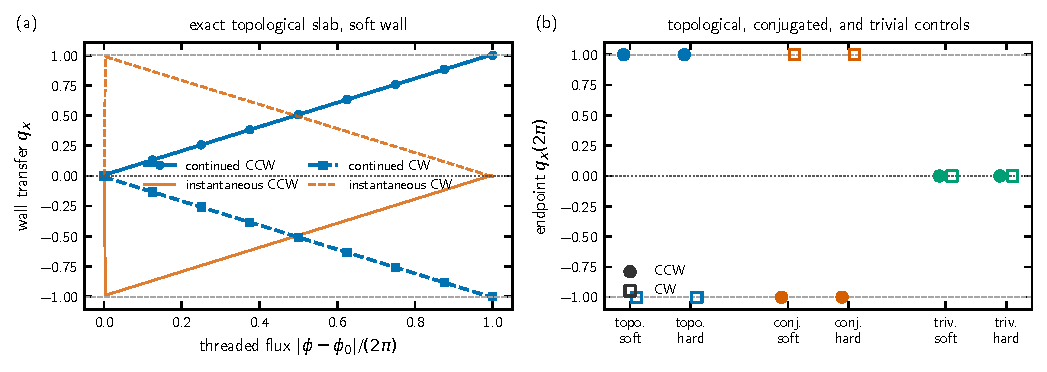
\includegraphics[width=\textwidth]{flux_threading_note_assets/figures/exact_flux_threading_controls.pdf}
 \caption{Exact flattened-Hamiltonian controls.  (a) Direct wall transfer
 $q_x$ for the soft-wall $C=+1$ slab.  The wall-continued projector reaches
 $+1$ for CCW and $-1$ for CW, whereas instantaneous energy refilling returns
 to zero after one flux quantum.  The apparent jump of the instantaneous
 curve occurs at the regulated wall crossing and represents immediate
 refilling, not dynamical charge motion.  (b) Endpoint responses for soft and
 hard topological, conjugated-Chern, and trivial controls.  Filled circles
 denote CCW and open squares CW.  The source real-space Chern markers are
 $+0.999958$, $-0.999958$, and zero, respectively.}
 \label{fig:exact-controls}
\end{figure*}

These controls separate a topological response from an algorithm which
merely prefers $|q_x|=1$.  Wall labeling does not produce a unit response in
the trivial state because there is no qualified topological wall doublet.
The Chern-conjugated control also shows that the sign is inherited from the
source topology, rather than inserted by the CCW/CW naming convention.

\section{Flux threading and spectral flow of monitored-trajectory endpoint states}

The completed result is shown in Figs.~\ref{fig:complete-histograms}--\ref{fig:mean-paths-dense} and
Table~\ref{tab:complete-endpoints}.  We retain the raw CCW and CW response of
every sample.  No direction-odd combination is used, and unresolved edge
clusters are not removed from the distribution.  The first fact visible in
the data is therefore particularly simple: the wall response is almost
binary.  CCW paths accumulate at $q_x=+1$, CW paths accumulate at $q_x=-1$,
and the principal departure is a much smaller peak at $q_x=0$.  Only about
0.2\% of all paths lie appreciably between those two alternatives.

\begin{figure*}[t]
 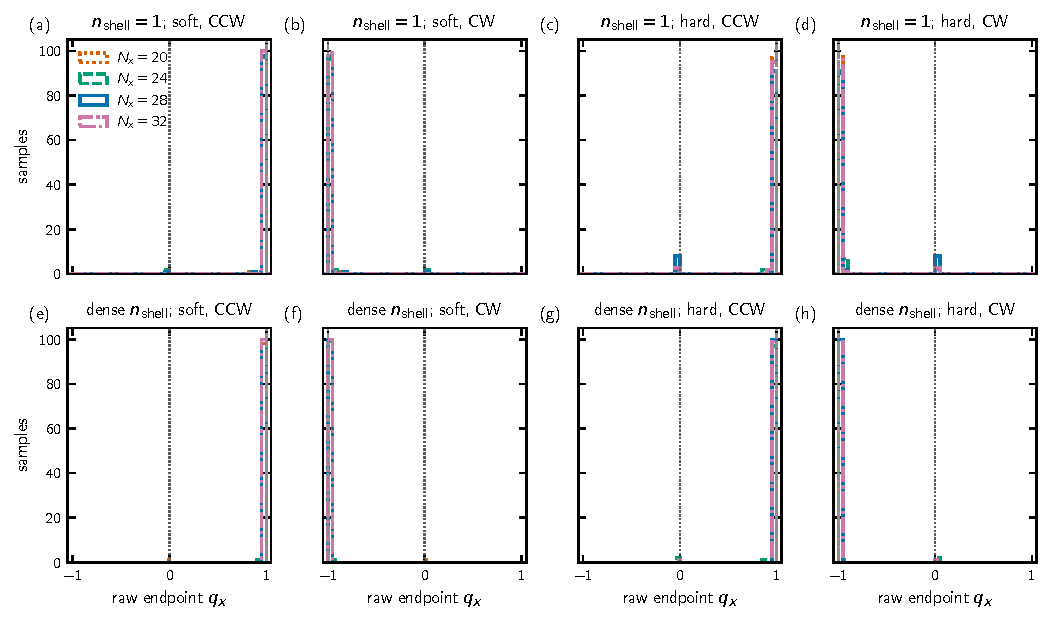
\includegraphics[width=\textwidth]{../results/N20_24_28_32x24_wall_diabatic_spectral_pump_reconciled_v1_v2/analysis/figures/reconciled_samplewise_wall_response_histograms.pdf}
 \caption{Sample-wise raw endpoint wall response for the completed monitored
 endpoint ensemble.  The upper row uses $n_{\rm shell}=1$ and the lower row
 uses the dense OW construction.  Columns show soft-wall CCW, soft-wall CW,
 hard-wall CCW, and hard-wall CW paths.  Each histogram contains $S=100$
 independent monitored endpoint states at fixed $N_x$; colors and line styles
 distinguish $N_x=20,24,28,32$.  Dashed vertical lines mark the
 orientation-expected values $q_x=+1$ (CCW) and $q_x=-1$ (CW), while dotted
 lines mark zero.  Unresolved paths are retained.  The distributions consist
 predominantly of a narrow unit-transfer peak with a small residual
 zero-transfer population, rather than a broad continuum of fractional
 charge.}
 \label{fig:complete-histograms}
\end{figure*}

\begin{figure*}[t]
 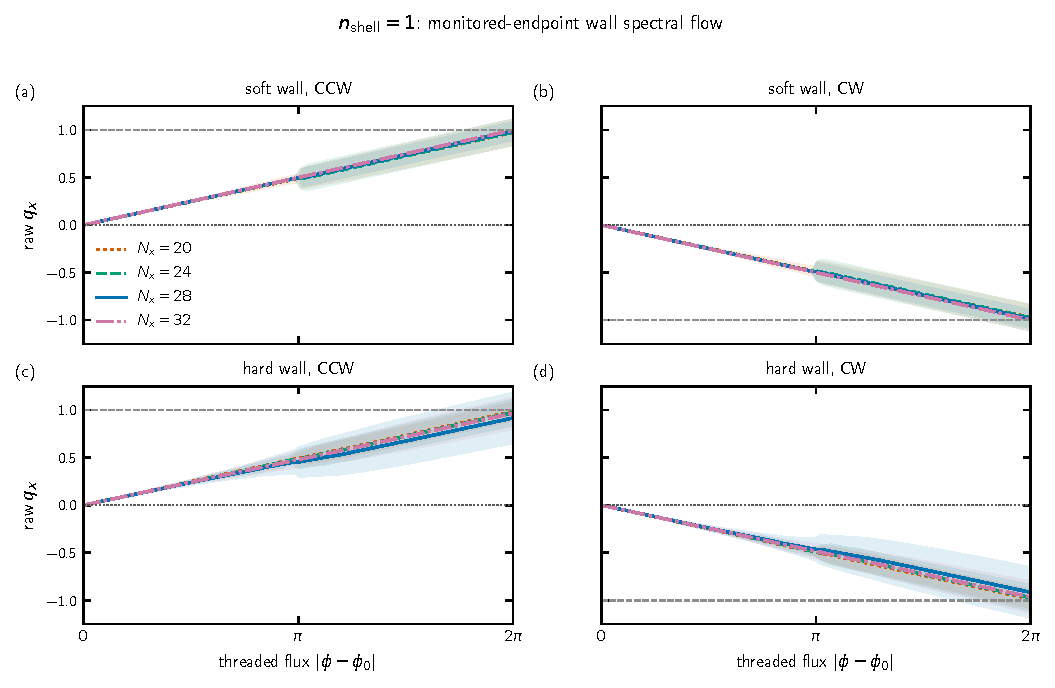
\includegraphics[width=\textwidth]{../results/N20_24_28_32x24_wall_diabatic_spectral_pump_reconciled_v1_v2/analysis/figures/reconciled_mean_qx_vs_flux_nsh1.pdf}
 \caption{Flux-resolved raw wall response for $n_{\rm shell}=1$.  Rows show
 soft and hard walls; columns show CCW and CW paths.  Each curve is the mean
 over $S=100$ independent monitored endpoint states and each shaded band is
 one trajectory standard deviation.  Colors and line styles distinguish
 $N_x=20,24,28,32$ at fixed $N_y=24$.  The horizontal dashed lines mark the
 orientation-expected unit responses, while dotted lines mark zero.  The
 horizontal coordinate is the nonnegative threaded distance
 $|\phi-\phi_0|$, so both directions run from zero to one flux quantum while
 remaining separate observables.  No direction-odd combination or removal
 of unresolved samples is used.}
 \label{fig:mean-paths-nsh1}
\end{figure*}

\begin{figure*}[t]
 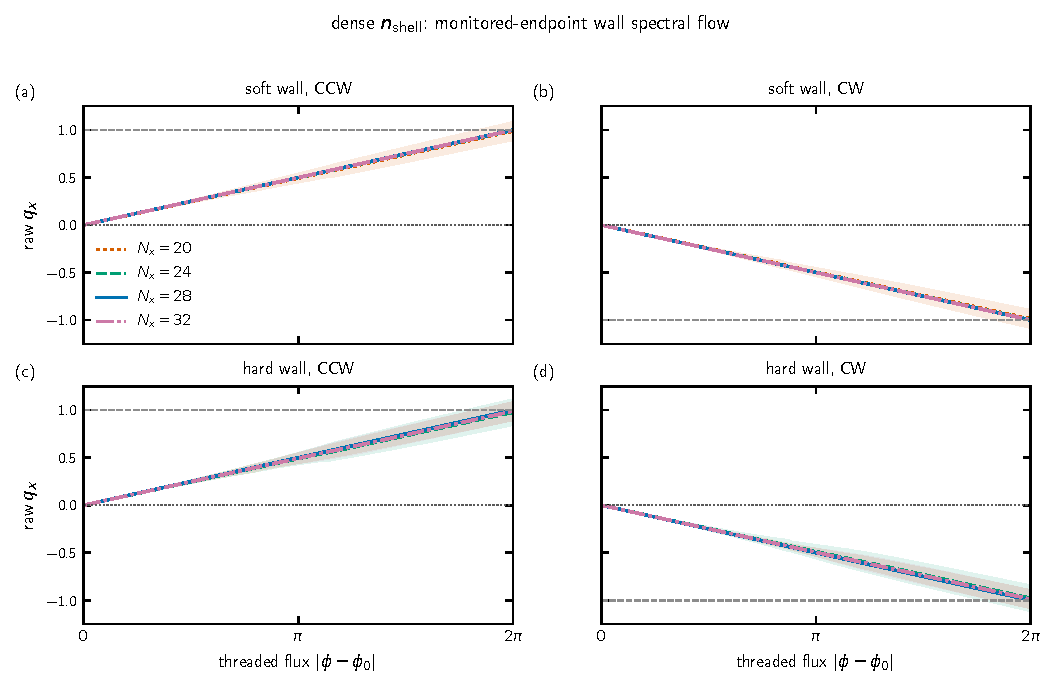
\includegraphics[width=\textwidth]{../results/N20_24_28_32x24_wall_diabatic_spectral_pump_reconciled_v1_v2/analysis/figures/reconciled_mean_qx_vs_flux_dense.pdf}
 \caption{Flux-resolved raw wall response for the dense OW construction, in
 the same format as Fig.~\ref{fig:mean-paths-nsh1}.  Every curve and band use
 the complete $S=100$ ensemble at that $(N_x,{\rm wall},{\rm direction})$
 cell.  The dense soft-wall curves at $N_x=28,32$ are nearly coincident and
 terminate at unit response with negligible trajectory spread; the other
 panels expose directly where the small zero-transfer subpopulation lowers
 the ensemble mean and enlarges its standard deviation.}
 \label{fig:mean-paths-dense}
\end{figure*}

\begin{table*}[t]
\caption{Completed raw endpoint response.  Every row contains $S=100$
independent monitored trajectories, and numbers in parentheses are trajectory
standard deviations.  The resolved percentage is the fraction satisfying
Eq.~\eqref{eq:qualification}.  The last column is the smaller of the raw CCW
and CW fractions satisfying $\sigma q_x>0.9$; it is descriptive and was not
used as an acceptance criterion.}
\label{tab:complete-endpoints}
\begin{ruledtabular}
\begin{tabular}{llrrrrr}
$n_{\rm shell}$ & wall & $N_x$ & $\langle q_x^{\rm CCW}\rangle$ &
$\langle q_x^{\rm CW}\rangle$ & resolved (\%) &
$\min_\sigma\Pr(\sigma q_x>0.9)$ (\%)\\
\hline
1 & soft & 20 & $+0.9749\,(0.1412)$ & $-0.9748\,(0.1408)$ & 97 & 97\\
1 & soft & 24 & $+0.9769\,(0.1406)$ & $-0.9768\,(0.1406)$ & 96 & 98\\
1 & soft & 28 & $+0.9884\,(0.1004)$ & $-0.9880\,(0.1010)$ & 97 & 98\\
1 & soft & 32 & $+0.9994\,(0.0043)$ & $-0.9993\,(0.0055)$ & 98 & 100\\
1 & hard & 20 & $+0.9853\,(0.1002)$ & $-0.9864\,(0.0999)$ & 99 & 99\\
1 & hard & 24 & $+0.9732\,(0.1413)$ & $-0.9737\,(0.1408)$ & 98 & 96\\
1 & hard & 28 & $+0.9177\,(0.2721)$ & $-0.9174\,(0.2720)$ & 92 & 92\\
1 & hard & 32 & $+0.9673\,(0.1714)$ & $-0.9676\,(0.1713)$ & 97 & 97\\
dense & soft & 20 & $+0.9884\,(0.1004)$ & $-0.9893\,(0.1000)$ & 99 & 99\\
dense & soft & 24 & $+0.9993\,(0.0064)$ & $-0.9993\,(0.0067)$ & 100 & 100\\
dense & soft & 28 & $+1.0000\,(0.0000)$ & $-1.0000\,(0.0000)$ & 100 & 100\\
dense & soft & 32 & $+1.0000\,(0.0000)$ & $-1.0000\,(0.0000)$ & 100 & 100\\
dense & hard & 20 & $+0.9896\,(0.1000)$ & $-0.9888\,(0.1002)$ & 99 & 99\\
dense & hard & 24 & $+0.9788\,(0.1409)$ & $-0.9792\,(0.1407)$ & 98 & 97\\
dense & hard & 28 & $+0.9996\,(0.0028)$ & $-0.9999\,(0.0007)$ & 100 & 100\\
dense & hard & 32 & $+0.9895\,(0.1000)$ & $-0.9893\,(0.1000)$ & 99 & 99\\
\end{tabular}
\end{ruledtabular}
\end{table*}

Of the 3200 directional paths, 3145 (98.3\%) have the correct orientation
and $|q_x|>0.9$; 3120 (97.5\%) lie in the narrower interval
$0.95\leq|q_x|\leq1.05$.  Forty-eight paths (1.5\%) lie within $0.1$ of
zero, leaving only seven paths between the near-zero and near-unit sectors.
The cleanest cells are the dense soft-wall ensembles at $N_x=28,32$, for
which all 200 directional paths per width reach the expected unit response
at the displayed precision.  The weakest cell is the $n_{\rm shell}=1$ hard
wall at $N_x=28$: eight of its 100 endpoint states close near zero in each
orientation, giving means $(+0.9177,-0.9174)$.  The hard-wall width trend is
therefore not monotone trajectory by trajectory, even though the $N_x=32$
cell recovers to 97\% correctly oriented paths above 0.9.

The numerical closure remains far below the sample-to-sample spread.  Across
the reconciled matrix, the maximum total-charge residual is
$4.55\times10^{-13}$, the maximum frame/projector residual is
$9.59\times10^{-14}$, and the largest forward--reverse undo error is
$2.33\times10^{-15}$.  The wall cluster is qualified for 1569 of the 1600
endpoint states.  Of the 31 unresolved states, 13 fail to isolate the edge
pair from neighboring modes and 10 fail the radius-two wall-weight threshold;
the remaining eight fail combinations involving the same isolation,
wall-weight, or polarization conditions.  These states remain in the raw
histograms and ensemble statistics.

\section{Comparison with the binary result}

The earlier ordinary-overlap experiment used the same endpoint states and
the same direct left/right subsystem charges.  At $N_x=20$ and
$n_{\rm shell}=1$, only 71\% of soft-wall and 36\% of hard-wall trajectories
had correctly oriented raw $|q_x|>0.5$.  At $N_x=24$, the corresponding
fractions were 91\% and 46\%.  For dense $N_x=20$ endpoints they were 86\%
and 84\%.  The wall-diabatized calculation raises these fractions to
98--99\% in the same completed cells, as shown in Fig.~\ref{fig:method-width}(a).

\begin{figure*}[t]
 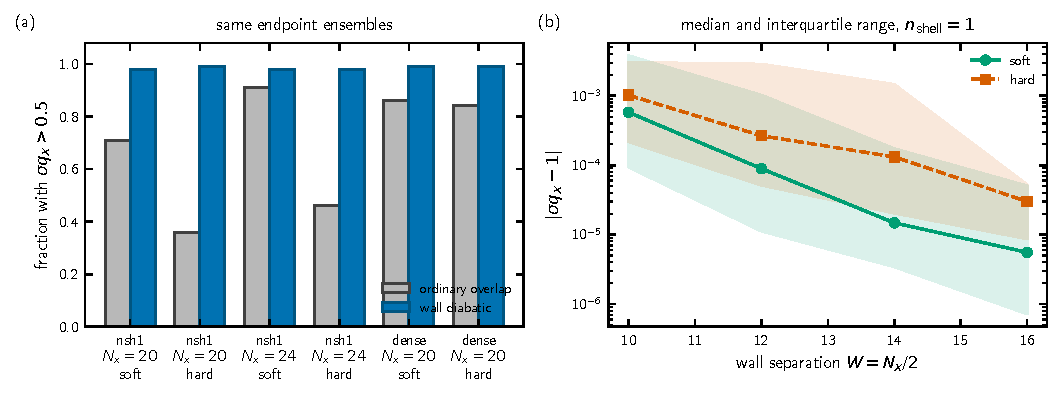
\includegraphics[width=\textwidth]{flux_threading_note_assets/figures/ordinary_overlap_vs_wall_diabatic_snapshot.pdf}
 \caption{Effect of the continuation rule and wall separation.  (a)
 Fraction of raw directional paths satisfying $\sigma q_x>0.5$ for the old
 ordinary-overlap rule and the wall-diabatized rule, evaluated on the same
 endpoint ensembles.  The improvement is methodological: the wall crossing
 is no longer delegated to a grid-sensitive global rank selector.  (b)
 Median $|\sigma q_x-1|$ for the $n_{\rm shell}=1$ wall-diabatized paths as a
 function of wall separation $W=N_x/2$; bands show the interquartile range.
 CW and CCW values are both included as raw directional observations.  This
 comparison figure records the earlier frozen analysis; the completed S100
 width distributions are given in Fig.~\ref{fig:complete-histograms}.}
 \label{fig:method-width}
\end{figure*}

The calculation did not become accurate because increasing $N_x$ made a
local phase act nonlocally.  Flux was already globally nontrivial through its
holonomy.  The large improvement came from defining the wall branch in a way
which matches the thermodynamic order of limits.  The old selector sometimes
followed the finite-size avoided crossing and sometimes jumped it, producing
the conspicuous zero/one distribution.  The new selector first verifies that
an isolated, oppositely localized doublet exists and then keeps its entering
wall label.  Once this choice is made, a qualified Chern wall pair is expected
to carry nearly one charge.

Increasing wall separation still matters.  For the soft wall, the median raw
quantization error decreases from $5.77\times10^{-4}$ at $W=10$ to
$5.56\times10^{-6}$ at $W=16$.  For the hard wall it decreases from
$1.02\times10^{-3}$ to $1.31\times10^{-4}$ between $W=10$ and $W=14$; the
completed $W=16$ value remains sharply concentrated near unit transfer.  This
is consistent with reduced inter-wall hybridization, but the resolved
fraction is not monotone: the complete hard-wall $N_x=28$ cell resolves 92\%,
less than the $N_x=20$ cell.  Trajectory-dependent mixing with additional
edge or bulk states therefore remains visible.  The completed dense
comparison strongly suppresses these exceptions, but four widths are still
insufficient for a controlled thermodynamic extrapolation of the unresolved
fraction.

\section{Interpretation and scope}

The result is a spectral pump of the flattened endpoint projector.  It says
that a monitored trajectory frequently contains an isolated wall doublet
whose Chern spectral-flow branch transfers one occupied mode across the
sample.  The exact control, orientation reversal, Chern-conjugation reversal,
trivial null response, large-gauge equivalence, and defect particle/hole pair
make this interpretation substantially sharper than observing $q_x\simeq1$
alone.

It is equally important to state what has not been shown.  The path
$P_{\rm wd}(\phi)$ is not obtained by evolving the monitored state in real
time.  The word \emph{diabatic} refers only to the internal wall splitting;
it does not mean that a fast physical quench was simulated.  An online
monitored ramp, a frozen measurement-record replay, and a Schr\"odinger ramp
sample different dynamical questions and need not reproduce this projector
path.  The present calculation diagnoses the branch which survives when the
wall separation is taken large before the flux rate is taken to zero.

Nor is a unit response imposed after the fact.  The fixed localization and
isolation thresholds are evaluated before using the wall label.  Failed
samples remain in the raw distributions, and the trivial control remains
zero.  Nevertheless, the method is deliberately targeted: once a qualified
two-wall cluster is found, preserving its wall label is the operational
definition of the thermodynamic spectral-flow branch.  The nontrivial
scientific outputs are therefore not only $q_x$, but also the fraction of
trajectories which possess such a cluster, its separation from spectators,
its wall leakage, its dependence on $N_x$ and $n_{\rm shell}$, and the Chern
marker of the source state.

\section{Conclusion}

Flux threading is a boundary-condition deformation with a local matrix
representation and a global holonomy.  A pure gauge rotation of the state
cannot change the subsystem charge; a genuine flux-threaded parent can carry
spectral flow because its eigenstate labels need not close after one flux
quantum.  In a finite two-wall geometry, the branch must be specified at the
avoided crossing.  Instantaneous refilling closes, ordinary global overlap is
mesh sensitive, and wall-diabatized continuation implements the
thermodynamic branch by treating the wall pair separately from the spectator
subspace.

The completed S100 matrix supports a robust, chirality-reversing, near-unit
spectral transfer in 98.3\% of the raw directional paths.  It also shows why
the earlier binary distributions were not simply a property of the charge
observable: they encoded an unstable branch choice.  The completed width
cells show a strong decrease of the quantization error with separation, while
the nonmonotone resolved fraction retains genuine sample dependence.  The
width and shell comparison must therefore report both quantities rather than
reducing the result to a single mean pump charge.

\clearpage
\appendix

\section{Completed-production provenance}

The 1595 immutable v1 pairs remain under
\path{results/N20_24_28_32x24_wall_diabatic_spectral_pump_s100_v1}.  The five
checksum-pinned numerical recoveries remain under
\path{results/N20_24_28_32x24_wall_diabatic_spectral_pump_numerical_recovery_v2}.
The recovery contract and its reason are recorded in
\path{WALL_DIABATIC_NUMERICAL_RECOVERY_V2.md}.  The completed table, endpoint histograms, and flux-resolved mean-path
figures are regenerated by
\path{analyze_wall_diabatic_reconciled_v1_v2.py}; its manifest and scalar
table are under
\path{results/N20_24_28_32x24_wall_diabatic_spectral_pump_reconciled_v1_v2/analysis}.
The earlier 920-pair working snapshot and its manifest are preserved under
\path{docs/flux_threading_note_assets} as a historical intermediate artifact,
but they are not used in Fig.~\ref{fig:complete-histograms} or
Table~\ref{tab:complete-endpoints}.  No production result, completion receipt,
checkpoint, or log is modified by the reconciled analysis.

An executable companion is provided at
\path{notebooks/equilibrium_wall_crossing_explorer/equilibrium_wall_crossing_explorer.ipynb}.
It rebuilds one translation-invariant $n_{\rm shell}=1$ equilibrium OW slab,
magnifies its finite-size wall crossing, and exposes flux sliders for the
energy eigenvalues, wall-resolved mode densities, instantaneous occupations,
continued occupations, and the resulting $q_x$.  The saved default run gives
$q_x(2\pi)=0.9999999992$ under overlap continuation and closes within
$3.5\times10^{-10}$ under instantaneous refilling.

\begin{thebibliography}{99}

\bibitem{Laughlin1981}
R. B. Laughlin, Quantized Hall conductivity in two dimensions,
Phys. Rev. B \textbf{23}, 5632 (1981).

\bibitem{NiuThouless1984}
Q. Niu and D. J. Thouless, Quantised adiabatic charge transport in the
presence of substrate disorder and many-body interaction,
J. Phys. A \textbf{17}, 2453 (1984).

\bibitem{Hatsugai1993}
Y. Hatsugai, Chern number and edge states in the integer quantum Hall effect,
Phys. Rev. Lett. \textbf{71}, 3697 (1993).

\bibitem{Kato1950}
T. Kato, On the adiabatic theorem of quantum mechanics,
J. Phys. Soc. Jpn. \textbf{5}, 435 (1950).

\end{thebibliography}

\end{document}
